\begin{center}
{\WorkType}
\\
Тема: {\Topic}
\\
Цель: Создание простейшей программы на языке Python с использованием QtQML. 
\end{center}
Задание:
Создание калькулятора.

Ход выполнения:
\begin{center}
Программа:
\end{center}
\begingroup
\fontsize{12pt}{12pt}\selectfont
\begin{verbatim}
from PyQt5.QtGui import QGuiApplication
from PyQt5.QtQml import QQmlApplicationEngine
from PyQt5.QtCore import QObject, pyqtSignal, pyqtSlot

class Calculator(QObject):
first_operand = ''
seond_operand = ''
g=False
def __init__(self):
QObject.__init__(self)

sumResult = pyqtSignal(float, arguments=['sum'])

subResult = pyqtSignal(float, arguments=['sub'])

clear=pyqtSignal(arguments=['C'])

@pyqtSlot()
def is_first(self):
return True

@pyqtSlot()
def clear(self):
self.first_operand=0.0 
self.g=False

@pyqtSlot(float,str)
def sub(self,c,sign):

self.sign=sign

if self.g==False:
self.first_operand = c
self.g=True
else:

self.sumResult.emit(self.first_operand - c)

@pyqtSlot(float,str)
def sum(self,c,sign):

self.sign=sign
if self.g==False:
self.first_operand = c
self.g=True
else:

self.sumResult.emit(self.first_operand + c)

@pyqtSlot(float,str)
def unmoj(self,c,sign):

self.sign=sign
if self.g==False:
self.first_operand = c
self.g=True
else:

self.sumResult.emit(self.first_operand * c)

@pyqtSlot(float,str)
def delen(self,c,sign):

self.sign=sign
if self.g==False:
self.first_operand = c
self.g=True
else:

self.sumResult.emit(self.first_operand / c)

@pyqtSlot(float)
def ravno(self,c):

if self.sign == "-":
a=self.first_operand - c
self.sumResult.emit(a)

self.first_operand=a 
elif self.sign == "+":
a=self.first_operand + c
self.sumResult.emit(a)

self.first_operand=a 
elif self.sign == "*":
a=self.first_operand * c
self.sumResult.emit(a)

self.first_operand=a 
elif self.sign == "/":
a=self.first_operand / c
self.sumResult.emit(a)

self.first_operand=a   

if __name__ == "__main__":
import sys

app = QGuiApplication(sys.argv)

engine = QQmlApplicationEngine()

calculator = Calculator()

engine.rootContext().setContextProperty("calculator", calculator)

engine.load("main.qml")

engine.quit.connect(app.quit)
sys.exit(app.exec_())


import QtQuick 2.5
import QtQuick.Controls 1.4
import QtQuick.Layouts 1.2

ApplicationWindow {
visible: true
width: 280
height: 300
title: qsTr("Калькулятор")
color: "whitesmoke"

// Input field of the first number
TextField {
id: sumResult
width: 260; 
height: 30;
x:10
y:10
}

Button {
text: qsTr ("0")
height: 40;
width: 50		   
x:10
y:50   

onClicked:{
sumResult.text+=("0")
}
}

Button {
text: qsTr ("1")
height: 40;
width: 50		   
x:80
y:50

onClicked:{
sumResult.text+=("1")
}
}

Button {
text: qsTr ("2")
height: 40;
width: 50		   
x:150
y:50

onClicked:{
sumResult.text+=("2")

}
}
Button {
text: qsTr ("3")
height: 40;
width: 50		   
x:10
y:100

onClicked:{
sumResult.text+=("3")
}
}
Button {
text: qsTr ("4")
height: 40;
width: 50		   
x:80
y:100

onClicked:{
sumResult.text+=("4")
}
}

Button {
text: qsTr ("5")
height: 40;
width: 50		   
x:150
y:100

onClicked:{
sumResult.text+=("5")
}
}
Button {
text: qsTr ("6")
height: 40;
width: 50		   
x:10
y:150

onClicked:{
sumResult.text+=("6")
}
}
Button {
text: qsTr ("7")
height: 40;
width: 50		   
x:80
y:150

onClicked:{
sumResult.text+=("7")
}
}
Button {
text: qsTr ("8")
height: 40;
width: 50		   
x:150
y:150

onClicked:{
sumResult.text+=("8")
}
}
Button {
text: qsTr ("9")
height: 40;
width: 50		   
x:10
y:200

onClicked:{
sumResult.text+=("9")
}
}
Button {
text: qsTr ("+")
height: 40;
width: 50		   
x:80
y:200
id: plus
onClicked:{

calculator.sum(sumResult.text,"+")
sumResult.text=("")
plus.enabled=false
min.enabled=false
umn.enabled=false
del.enabled=false
}
}
Button {
text: qsTr ("-")
height: 40;
width: 50		   
x:150
y:200
id: min 
onClicked:{
calculator.sub(sumResult.text,"-")
sumResult.text=("")
plus.enabled=false
min.enabled=false
umn.enabled=false
del.enabled=false
}
}
Button {
text: qsTr ("*")
height: 40;
width: 50		   
x:220
y:200
id: umn
onClicked:{

calculator.unmoj(sumResult.text,"*")
sumResult.text=("")
plus.enabled=false
min.enabled=false
umn.enabled=false
del.enabled=false
}
}
Button {
text: qsTr ("/")
height: 40;
width: 50		   
x:220
y:150
id: del
onClicked:{

calculator.delen(sumResult.text,"/")
sumResult.text=("")
plus.enabled=false
min.enabled=false
umn.enabled=false
del.enabled=false
}
}

Button {
text: qsTr ("CE")
height: 90;
width: 50		   
x:220
y:50

onClicked:{
calculator.clear()
sumResult.text=("")
}
}
Button {
text: qsTr ("=")
height: 40;
width: 260		   
x:10
y:250

onClicked:{

calculator.ravno(sumResult.text)
plus.enabled=true
min.enabled=true
umn.enabled=true
del.enabled=true
}		
}
Connections {
target: calculator

// Sum signal handler
onSumResult: {
// sum was set through arguments=['sum']
sumResult.text = sum
}

// Subtraction signal handler
onSubResult: {
// sub was set through arguments=['sub']
subResult.text = sub	  
}
}
}
\end{verbatim}
\endgroup
Изображен код программы калькулятор.
\begin{center}
Результат работы программы:
\end{center}

\begin{figure}[h]
	\centering
	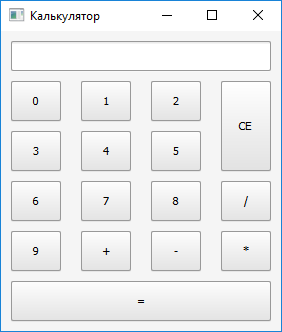
\includegraphics[scale=1]{s1}

	\label{fig:s1}
\end{figure}


Вывод: Был создан калькулятор на python с использованием QtQml. 



